\documentclass{article}
\usepackage[utf8]{inputenc}
\usepackage{amssymb}
\usepackage{amsfonts}
\usepackage{amsmath}
\usepackage[utf8]{inputenc}
\usepackage[english]{babel}
\usepackage{lmodern}
\usepackage{float}
\usepackage{graphicx}
\DeclareGraphicsExtensions{.eps,.pdf,.png,.jpg}
\usepackage{latexsym}
\usepackage{hyperref}
\usepackage[euler]{textgreek}
\usepackage{stackengine}
\usepackage{listings}
\usepackage[version-1-compatibility]{siunitx}
\usepackage[usenames,dvipsnames]{xcolor}
\usepackage{pdfpages}
\hypersetup{pdfborder={0 0 0}}
\usepackage{pgfplots}
\pgfplotsset{compat=newest}
\pgfplotsset{plot coordinates/math parser=false}
\newlength\figureheight
\newlength\figurewidth
\usepackage[section]{placeins}%Sørger for at plots og andre floats holder seg til sin section.
\lstset{flexiblecolumns=true}


\lstloadlanguages{Matlab}
\setlength\parindent{0pt}%Setter indent til 0
\definecolor{MyDarkGreen}{rgb}{0.0,0.4,0.0}


\lstloadlanguages{Matlab}%
\lstset{language=Matlab,                        % Use MATLAB
        frame=single,                           % Single frame around code
        basicstyle=\small\ttfamily,             % Use small true type font
        keywordstyle=[1]\color{Blue}\bfseries,        % MATLAB functions bold and Blue
        keywordstyle=[2]\color{Orchid},         % MATLAB function arguments Orchid
        keywordstyle=[3]\color{Blue}\underbar,  % User functions underlined and Blue
        identifierstyle=,                       % Nothing special about identifiers
        % Comments small dark green courier
        commentstyle=\usefont{T1}{pcr}{m}{sl}\color{MyDarkGreen}\small,
        stringstyle=\color{Orchid},             % Strings are Orchid
        showstringspaces=false,                 % Don't put marks in string spaces
        tabsize=5,                              % 5 spaces per tab
        %
        %%% Put standard MATLAB functions not included in the default
        %%% language here
        morekeywords={xlim,ylim,var,alpha,factorial,poissrnd,normpdf,normcdf},
        %
        %%% Put MATLAB function parameters here
        morekeywords=[2]{on, off, interp},
        %
        %%% Put user defined functions here
        morekeywords=[3]{FindESS, homework_example},
        %
        morecomment=[l][\color{Blue}]{...},     % Line continuation (...) like Blue comment
        numbers=left,                           % Line numbers on left
        firstnumber=1,                          % Line numbers start with line 1
        numberstyle=\tiny\color{Blue},          % Line numbers are Blue
        stepnumber=5                            % Line numbers go in steps of 5
        }

% Includes a MATLAB script.
% The first parameter is the label, which also is the name of the script
%   without the .m.
% The second parameter is the optional caption.
\newcommand{\matlabscript}[2]{\begin{itemize}\item[]\lstinputlisting[caption=#2,label=#1]{#1.m}\end{itemize}}


\title{Exercise 3 - TTK4130 Modeling and Simulation}
\author{Camilla Sterud}
\date{}

\begin{document}

\maketitle

\newpage

\section{Problem 1}

Volterra-Lotka predator-prey model:

\begin{align} \label{eq:volterralotka}
    \dot u &= u(v-3) \\
    \dot v &= v(2-u)\nonumber
\end{align}

"Energy" function

\begin{equation*}
    V = u - 2\ln(u) + v - 3\ln(v)
\end{equation*}

\subsection{a}

\begin{equation*}
    \dot V = \frac{\partial V}{\partial u}\dot u + \frac{\partial V}{\partial v}\dot v
\end{equation*}

Calculate the partial derivatives of $V$ and inserting the equations \ref{eq:volterralotka} gives us

\begin{equation*}
    \dot V = (1-\frac{2}{u})u(v-3) + (1 - \frac{3}{v})v(2-u) = 0,
\end{equation*}

which means that $V$ is constant for solutions of the system \ref{eq:volterralotka}. This means that the system is stable and will not grow to $\pm\infty$.

\subsection{b}

As seen in Figure \ref{fig:1b} the number of foxes and rabbits is periodic and $V$ is constant. 

\begin{figure}[H]
    \centering
    \includegraphics[width = 0.8\textwidth]{ex6_1b}
    \caption{The system from \ref{eq:volterralotka} simulated in Dymola with $(u_0,v_0) = (1,4)$.}
    \label{fig:1b}
\end{figure}



\subsection{c}

Want to linearize the system around $(u^*,v^*) = (2,3)$, so $\Delta u = u-u^*, \: \Delta v = v - v^*, \: \dot u = f_1, \: \dot v = f_2$.

\begin{align*}
    \Delta \dot u &= \left. \frac{\partial f_1}{\partial u} \right.\bigg|_{\shortstack{\tiny $u = u^*$ \\ \tiny $v = v^*$}} \Delta u + \left. \frac{\partial f_1}{\partial v} \right.\bigg|_{\shortstack{\tiny $u = u^*$ \\ \tiny $v = v^*$}} = 2(v-3)\\
    \Delta \dot v &= \left. \frac{\partial f_2}{\partial u} \right.\bigg|_{\shortstack{\tiny $u = u^*$ \\ \tiny $v = v^*$}} \Delta u + \left. \frac{\partial f_2}{\partial v} \right.\bigg|_{\shortstack{\tiny $u = u^*$ \\ \tiny $v = v^*$}} = 3(2-u) 
\end{align*}

This yields the linearized system

\begin{equation}\label{eq:linearizedvt}
    \begin{bmatrix}
        \dot u\\ \dot v
    \end{bmatrix} = 
    \begin{bmatrix}
        0 & 2 \\ -3 & 0
    \end{bmatrix}
    \begin{bmatrix}
        u\\ v
    \end{bmatrix} +
    \begin{bmatrix}
        -6\\6
    \end{bmatrix}.
\end{equation}

This system has the eigevalues $\lambda = \pm i\sqrt {6}$, so the linearized system is marginally stable.

\begin{figure}[H]
    \centering
    \includegraphics[width = 0.8\textwidth]{ex6_1c_23}
    \caption{The linearized system from \ref{eq:linearizedvt} simulated in Dymola with $(u_0,v_0) = (2,3)$.}
    \label{fig:1c_23}
\end{figure}

\begin{figure}[H]
    \centering
    \includegraphics[width = 0.8\textwidth]{ex6_1c_202_298}
    \caption{The linearized system from \ref{eq:linearizedvt} simulated in Dymola with $(u_0,v_0) = (2.02,2.98)$.}
    \label{fig:1c_202_298}
\end{figure}

\begin{figure}[H]
    \centering
    \includegraphics[width = 0.8\textwidth]{ex6_1c_19_31}
    \caption{The linearized system from \ref{eq:linearizedvt} simulated in Dymola with $(u_0,v_0) = (1.9,3.1)$.}
    \label{fig:1c_19_31}
\end{figure}

When simulating the linearized system with intital conditions $(u_0,v_0) = (2,3)$, as seen in Figure \ref{fig:1c_23}, the solution is constant. When simulated with initial values with slight deviations from the equilibrium, as seen in figures \ref{fig:1c_202_298} and \ref{fig:1c_19_31} the linearized system is an oscillator with frequency close to $f = \frac{\sqrt{6}}{2\pi}$

\subsection{d}

The code for this excercise can be seen in Listing 1. From the phase plots in figures \ref{fig:1d_ee} to \ref{fig:1d_imr} and the plots of the "energy" in figures \ref{fig:1d_vee} and \ref{fig:1d_v}, we see that the explicit Euler method is unstable, while the implicit Euler method and the implicit midpoint rule are stable for this system with $h = 0.1$. For smaller $h$, the implicit Euler method has a constant $V$, but the explicit Euler method is unstable for all $h$ when simulating this system.


\begin{figure}[H]
    \centering
    \includegraphics[width = 0.8\textwidth]{modsim_ex6_1d_ee}
    \caption{Phase plot of the system \ref{eq:volterralotka} simulated with the explicit Euler method.}
    \label{fig:1d_ee}
\end{figure}

\begin{figure}[H]
    \centering
    \includegraphics[width = 0.8\textwidth]{modsim_ex6_1d_ie}
    \caption{Phase plot of the system \ref{eq:volterralotka} simulated with the implicit Euler method.}
    \label{fig:1d_ie}
\end{figure}

\begin{figure}[H]
    \centering
    \includegraphics[width = 0.8\textwidth]{modsim_ex6_1d_imr}
    \caption{Phase plot of the system \ref{eq:volterralotka} simulated with the implicit midpoint rule.}
    \label{fig:1d_imr}
\end{figure}

\begin{figure}[H]
    \centering
    \includegraphics[width = 0.8\textwidth]{modsim_ex6_1d_v}
    \caption{The "energy" of the system \ref{eq:volterralotka} when simulated with the explicit Euler method.}
    \label{fig:1d_vee}
\end{figure}


\begin{figure}[H]
    \centering
    \includegraphics[width = 0.8\textwidth]{modsim_ex6_1d_vee}
    \caption{The "energy" of the system \ref{eq:volterralotka} when simulated with the implicit Euler method adn midpoint rule.}
    \label{fig:1d_v}
\end{figure}

\matlabscript{ModSim_ex6_1d}{Code for simulating the system from \ref{eq:volterralotka} in MATLAB with Euler and implicit Euler and implicit midpoint rule methods.}

\section{Problem 2}

\subsection{a}

Lobatto IIIA has stability function $R(s) = P_m^m(s)$. 
From the book we know that $|P_m^k(s)| \leq 1 \: \forall \: Re(s) \leq 0, \: k\leq m \leq k+2$.
A method is A-stable if $|R(h\lambda)| \leq 1 \: \forall \: Re(h\lambda) \leq 0$, so by replacing $s$ with $h\lambda$ and since $k=m$ for Lobatto IIIA, we see that it is clearly A-stable.

\subsection{b}

A method is L-stable if it is A-stable and $\lim_{\omega\to \infty}|R(hj\omega)| = 0$.

\begin{align*}
    \lim_{\omega\to \infty}|R(hj\omega)| &=\frac{|1 + \gamma_1j\omega h + ... +\gamma_m(j\omega h)^m|}{|1 + \beta_1j\omega h + ... + \beta_m(j\omega h)^m|} \\
    &= \frac{|\gamma_m|}{|\beta_m|} \neq 0,
\end{align*}

so Lobatto IIIA is not L-stable.

\section{Problem 3}

\begin{table}
\centering
\begin{tabular}{c|c c}\label{tab:butcher}
    $0$ & $\frac{1}{4}$ & $-\frac{1}{4}$ \\
    $\frac{2}{3}$ & $\frac{1}{4}$ & $\frac{5}{12}$ \\
    \hline
        & $\frac{1}{4}$ & $\frac{3}{4}$
\end{tabular}
\caption{Butcher array for Runge-Kutta method.}
\end{table}

\subsection{a}

The method is implicit. This can be seen from the butcher array, as it is not lower triangular.

\subsection{b}
Fromt the butcher array it can be seen that 

\begin{align*}
    \mathbf{A} &= 
    \begin{bmatrix}
        \frac{1}{4} & -\frac{1}{4} \\
        \frac{1}{4} & \frac{5}{12}
    \end{bmatrix}\\
    \mathbf{b} &= \begin{bmatrix}
        \frac{1}{4} \\
        \frac{3}{4}
    \end{bmatrix}
\end{align*}

From the book we know that 

\begin{equation*}
    R(h\lambda) = (1 + h\lambda\mathbf{b}^T(\mathbf{I} - h\lambda\mathbf{A})^{-1}\mathbf{1}).
\end{equation*}

Inserting and calculating yields

\begin{equation*}
    \underline{\underline{R(h\lambda) = \frac{1 + \frac{1}{3}h\lambda}{1 - \frac{2}{3}h\lambda + \frac{1}{6}(h\lambda)^2} = P_2^1(h\lambda)}}
\end{equation*}

\subsection{c}

This method is L-stable according to Theorem (14.6.5) in the book, since $m=k+1$. Therefore it is also A-stable.

\section{Problem 4}
\subsection{a}

\begin{align*}
    \dot m &= -\rho q\\
    q &= C_v\sqrt{p-p_0} = C_v\sqrt{\rho g h}\\
    \dot m &= \dot h A\rho
\end{align*}

\begin{equation}\label{eq:tank}
    \underline{\underline{\dot h = -\frac{C_v}{A}\sqrt{\rho g h}}}
\end{equation}

\subsection{b}

\begin{equation*}
    \underline{\underline{\Delta \dot h = \left. \frac{\partial (\dot h)}{\partial h} \right.\bigg|_{\shortstack{$h = h^*$}} \Delta h
    = -\frac{C_v\rho g}{2A\sqrt{\rho g h^*}}\Delta h}}
\end{equation*}

This linearized system had eigenvalue $\lambda = -\frac{C_v\rho g}{2A\sqrt{\rho g h^*}}$ which approaches $-\infty$ as $h^* \rightarrow 0$.

\subsection{c}

ode45 implements a Runge-Kutta method with variable step length. A seen in Figure \ref{fig:4c} the steplength is very small in towards the end of the simulation, where $h \rightarrow 0$. The code for simulating this system can be seen in Listing 2.

\begin{figure}[H]
    \centering
    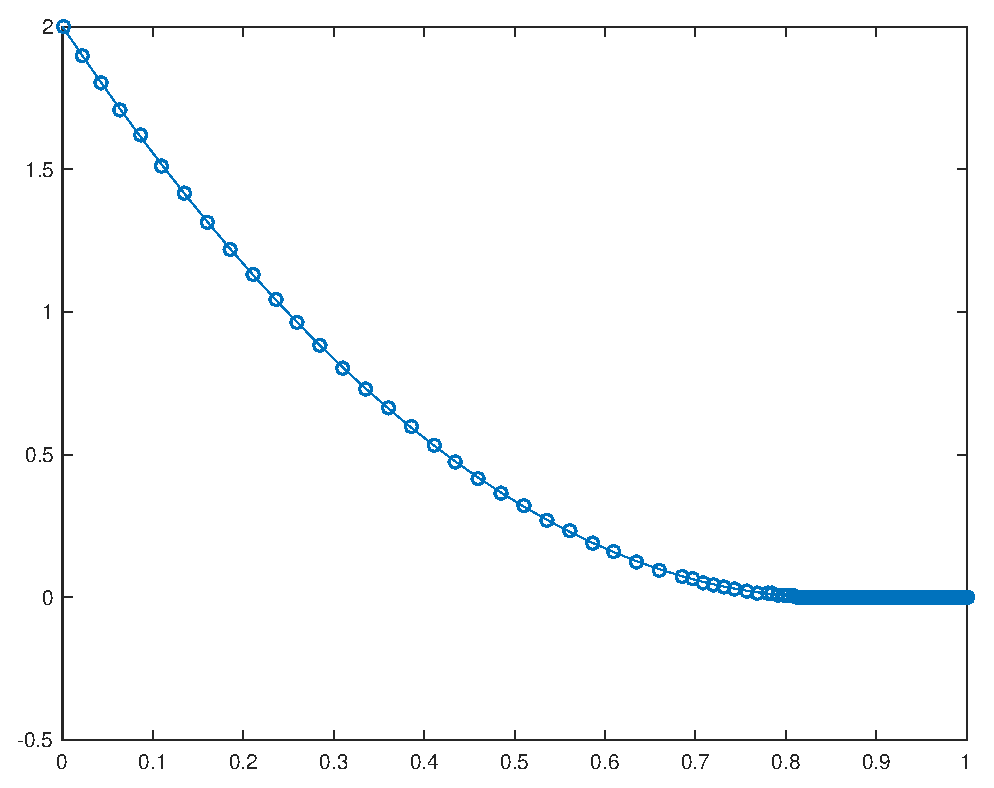
\includegraphics[width = 0.8\textwidth]{modsim_ex6_4c}
    \caption{The system from Equation \ref{eq:tank} simulated in MATLAB using ode45.}
    \label{fig:4c}
\end{figure}

\matlabscript{modsim_ex6_4c}{4c}



\end{document}